%%%%%%%%%%%%%%%%%%%%%%%%%%%%%%%%%%%%%%%%%%%%%%%%%%%%%%%%%%%%%%%%%%%%%%
% Overleaf (WriteLaTeX) Example: Molecular Chemistry Presentation
%
% Source: http://www.overleaf.com
%
% In these slides we show how Overleaf can be used with standard
% chemistry packages to easily create professional presentations.
%
% Feel free to distribute this example, but please keep the referral
% to overleaf.com
%
%%%%%%%%%%%%%%%%%%%%%%%%%%%%%%%%%%%%%%%%%%%%%%%%%%%%%%%%%%%%%%%%%%%%%%

\documentclass[xcolor={dvipsnames}]{beamer}

\mode<presentation>
{
  \usetheme{Madrid}       % or try default, Darmstadt, Warsaw, ...
  \usecolortheme{default} % or try albatross, beaver, crane, ...
  \usefonttheme{default}    % or try default, structurebold, ...
  \setbeamertemplate{navigation symbols}{}
  \setbeamertemplate{caption}[numbered]
}

\usepackage[english]{babel}
\usepackage[utf8x]{inputenc}
\usepackage{graphicx}
\usepackage{hyperref}
  \hypersetup{colorlinks=true}
  \hypersetup{urlcolor=blue}
  \hypersetup{linkcolor = .}
\usepackage{xcolor}
\usepackage{siunitx}
  \sisetup{separate-uncertainty = true}
\DeclareSIUnit\barn{b}
\usepackage{physics}
\usepackage[font=small,labelfont=bf]{caption}
\usepackage{subcaption}
\usepackage[en-GB]{datetime2}
\usepackage{overpic}
\usepackage{feynmp}
\DeclareGraphicsRule{*}{mps}{*}{}
\usepackage{scalerel}
\newcommand{\mylbrace}[2]{\vspace{#2pt}\hspace{6pt}\scaleleftright[\dimexpr5pt+#1\dimexpr0.06pt]{\lbrace}{\rule[\dimexpr2pt-#1\dimexpr0.5pt]{-4pt}{#1pt}}{.}}
\newcommand{\myrbrace}[2]{\vspace{#2pt}\scaleleftright[\dimexpr5pt+#1\dimexpr0.06pt]{.}{\rule[\dimexpr2pt-#1\dimexpr0.5pt]{-4pt}{#1pt}}{\rbrace}\hspace{6pt}}

% Trim in percent
\usepackage{adjustbox}

% No "Figure" prefix
\setbeamertemplate{caption}{\raggedright\insertcaption\par}

% Nice decay amplitude diagrams
\usepackage{amsmath,amssymb,tikz-cd}

% Strike out text
\usepackage[normalem]{ulem}

% For figures with text overlay
\usepackage{overpic}

% Arrows
\usepackage{tikz}
\newcommand{\tikzmark}[1]{\tikz[remember picture] \node[coordinate] (#1) {#1};}

% Colourbox with line breaks
\newcommand{\cbox}[2][lime!20]{%
  \colorbox{#1}{\parbox{\dimexpr\linewidth-2\fboxsep}{\strut #2\strut}}%
}

% Vector arrows
\usepackage[pdftex]{pict2e}

% Checkmark symbol
\def\checkmark{\tikz\fill[scale=0.4](0,.35) -- (.25,0) -- (1,.7) -- (.25,.15) -- cycle;}

% Here's where the presentation starts, with the info for the title slide
\title[RTA WP2 meeting]{First look at updated HLT2 forward tracking parameterisations}

\author[Martin Tat]{Martin Tat}
\institute[Heidelberg]{Heidelberg University}
\date{6th May 2025}

\titlegraphic{
\includegraphics[height = 2.3cm]{lhcb.jpg}\hspace{1.0cm}~%
              
\includegraphics[height = 2.3cm]{HeidelbergLogo.pdf}}

\begin{document}

\begin{frame}
  \titlepage
\end{frame}

% These three lines create an automatically generated table of contents.
\begin{frame}{Outline}
  \tableofcontents
\end{frame}

\section{Introduction}

\begin{frame}{Introduction}
  \vspace{0.0cm}
  {\Large I've had a look at the HLT2 forward tracking algorithm}
  \vspace{0.5cm}
  \begin{itemize}
    \setlength\itemsep{1.0em}
    \item{Relevant code lives in \texttt{Rec/Pr/PrAlgorithms/src/}}
    \begin{itemize}
      \item{\texttt{PrForwardTracking.cpp}}
      \item{\texttt{PrTrackModel.cpp}}
    \end{itemize}
    \item{Tracking algorithm described in three steps:}
    \begin{enumerate}
      \item{Trajectories based on equations of motion and detector geometry}
      \item{Parameterise complex calculations using polynomials}
      \item{Determine coefficients by fits to MC}
    \end{enumerate}
    \item{I plan to update these parameterisations}
    \begin{itemize}
      \item{Previous work based on MC from 2019 (\texttt{DC19})}
      \item{New magnetic field map (presented \href{https://indico.cern.ch/event/1539235/\#3-update-magnetic-field-map}{here})}
    \end{itemize}
  \end{itemize}
\end{frame}

\begin{frame}{Introduction}
  \vspace{0.0cm}
  {\Large Based on work by Andre G{\"u}nther\\}
  {\large Many thanks to Andre for the extensive documentation!}
  \vspace{0.5cm}
  \begin{itemize}
    \setlength\itemsep{1.0em}
    \item{Algorithm described in his thesis: \href{https://cds.cern.ch/record/2865000?ln=en}{CERN-THESIS-2023-097}}
    \begin{itemize}
      \item{All parameterisations are explained thoroughly}
      \item{Numerical results all agree with what is in Rec}
    \end{itemize}
    \item{Code available in: \href{https://gitlab.cern.ch/gunther/prforwardtracking-parametrisation-tuner}{Reco-Parameterisation-Tuner}}
    \begin{itemize}
      \item{Only minor changes required to get code running with latest environment}
      \item{All parameterisations can be reproduced with files found on Heidelberg computing cluster}
      \item{Moore scripts provided for rerunning with new MC (must be XDIGI)}
    \end{itemize}
  \end{itemize}
\end{frame}

\section{Overview of forward tracking algorithm}

\begin{frame}{Overview of forward tracking algorithm}
  \vspace{0.0cm}
  \begin{figure}[htb]
    \centering
    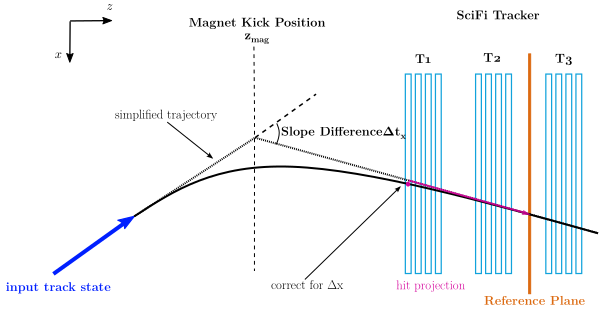
\includegraphics[width=0.75\textwidth]{Plots/MagnetKinkPosition.png}
    \caption*{\small From CERN-THESIS-2023-097}
  \end{figure}

  \begin{itemize}
    \item{Simplified track model: Assume magnet ``kicks'' particle at $z = z_{\rm mag}$}
    \item{Parameterise $z_{\rm mag}$ as:}
  \end{itemize}
  \begin{equation*}
    z_{\rm mag} = c_0 + c_1t_x^2 + c_3t_y^2 + \Delta t_x^\prime(c_2t_x + c_4\Delta t_x^\prime)
  \end{equation*}
\end{frame}

\begin{frame}{Overview of forward tracking algorithm}
  \vspace{0.0cm}
  \begin{figure}[htb]
    \centering
    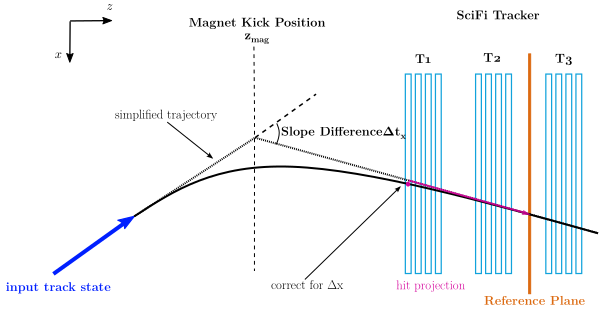
\includegraphics[width=0.75\textwidth]{Plots/MagnetKinkPosition.png}
    \caption*{\small From CERN-THESIS-2023-097}
  \end{figure}
  \begin{itemize}
    \item{True path in $xz$ plane deviates due to the SciFi fringe field}
    \item{Parameterise trajectory as:}
  \end{itemize}
  \begin{equation*}
    x(z) = a_x + b_x(z - z_{\rm ref}) + c_x(z - z_{\rm ref})^2 + d_x(z - z_{\rm ref})^3
  \end{equation*}
\end{frame}

\begin{frame}{Overview of forward tracking algorithm}
  \vspace{0.0cm}
  \begin{figure}[htb]
    \centering
    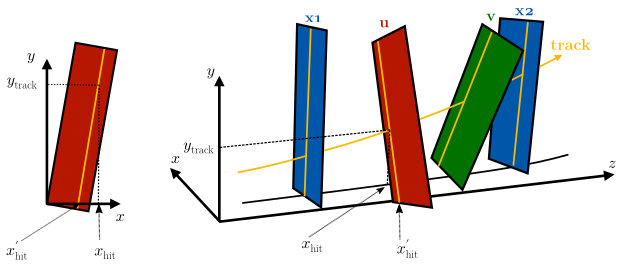
\includegraphics[width=0.7\textwidth]{Plots/StereoAngleCorrection.png}
    \caption*{\small From CERN-THESIS-2023-097}
  \end{figure}
  \begin{itemize}
    \item{Hits in stereo layers must be ``rotated'', which requires $y$-position}
    \item{Account for small track curvature in $yz$ plane:}
  \end{itemize}
  \begin{align*}
    y_{\rm corr}^L =& \Delta t_x(c_0^L + c_2^Lt_xt_y + c_5^Lt_xt_y^3 + c_6^Lt_x^3t_y) \\
    +& t_x(c_1^L + c_3^Lt_xt_y + c_4^Lt_xt_y^3 + c_7^Lt_x^3t_y)
  \end{align*}
\end{frame}

\begin{frame}{Overview of forward tracking algorithm}
  \vspace{0.0cm}
  \begin{figure}[htb]
    \centering
    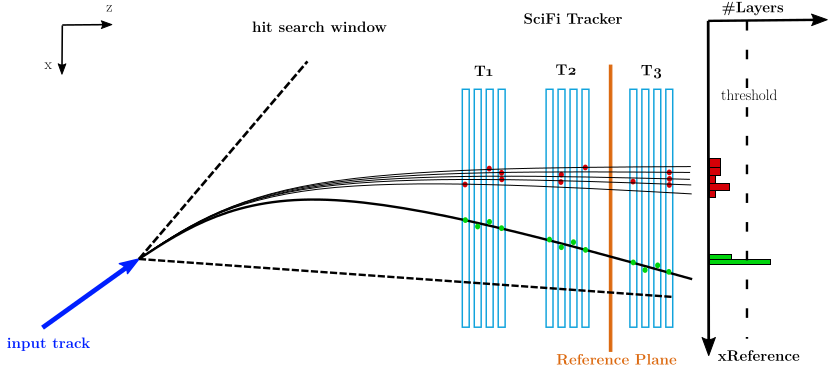
\includegraphics[width=1\textwidth]{Plots/HoughTransform.png}
  \caption*{\small From CERN-THESIS-2023-097}
  \end{figure}
  \vspace{-0.3cm}
  \begin{itemize}
    \item{Once all SciFi hits are parameterised, map hits to reference plane}
    \item{Hits from real tracks show peaks in ``Hough histogram''}
  \end{itemize}
\end{frame}

\begin{frame}{Overview of forward tracking algorithm}
  \vspace{0.0cm}
  \begin{figure}[htb]
    \centering
    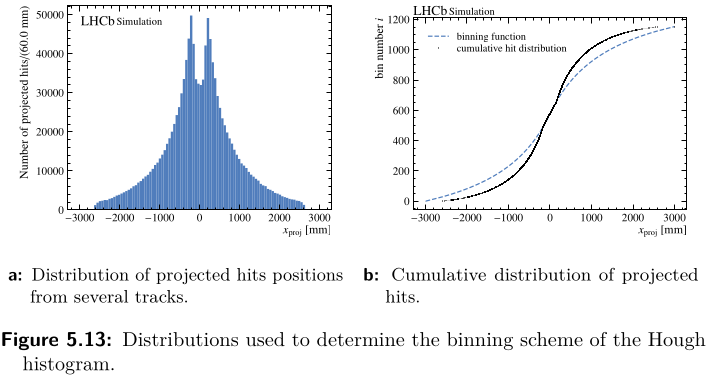
\includegraphics[width=0.7\textwidth]{Plots/HoughDistribution.png}
  \caption*{\small From CERN-THESIS-2023-097}
  \end{figure}
  \vspace{-0.3cm}
  \begin{itemize}
    \item{Hits (in reference plane) are not uniform along $x$-axis}
    \item{Transform $x$ by sigmoid function before binning:}
  \end{itemize}
  \begin{equation*}
    p_0 + \frac{p_1x_{\rm proj}}{1 + p_2\lvert x_{\rm proj}\rvert}
  \end{equation*}
\end{frame}

\begin{frame}{Overview of forward tracking algorithm}
  \vspace{0.0cm}
  \begin{figure}[htb]
    \centering
    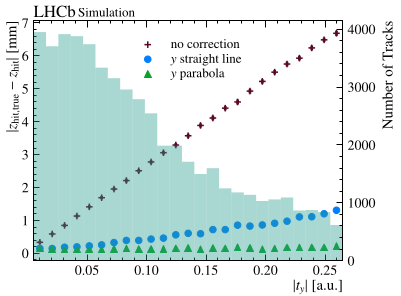
\includegraphics[width=0.5\textwidth]{Plots/yCorrectionPerformance.png}
  \caption*{\small From CERN-THESIS-2023-097}
  \end{figure}
  \vspace{-0.3cm}
  \begin{itemize}
    \item{$z$-position must then be corrected for small tilt in $yz$ plane}
    \item{Assume trajectory in $yz$ plane is a parabola:}
  \end{itemize}
  \begin{align*}
    y(z) =& a_y + b_y(z - z_{\rm ref}) + c_y(z - z_{\rm ref})^2 \\
    z_{\rm hit}^\prime =& z_{\rm hit} + \tan(0.21^\circ)y(z)
  \end{align*}
\end{frame}

\begin{frame}{Overview of forward tracking algorithm}
  \vspace{0.0cm}
  {\large Finally, obtain momentum from change in track slope $\Delta t_x$:}
  \vspace{0.2cm}
  \begin{equation*}
    \frac{q}{p} = \frac{\Delta t_x}{r_IB_{\rm int}}
  \end{equation*}
  \vspace{1.0cm}
  {\\~\large The field integral $B_{\rm int}$ is parameterised as:}
  \begin{align*}
    B_{\rm int} =& c_0 + t_y^2(c_1 + c_5t_y^2 + c_6t_x^2) + t_xb_x(c_{10}t_x + c_3 + c_7t_y^2) \\
    +& c_{11}b_x^4 + c_2t_x^2 + b_x^2(c_4 + c_8t_y^2) + c_9t_x^4
  \end{align*}
\end{frame}

\begin{frame}{Overview of forward tracking algorithm}
  \vspace{0.0cm}
  {\large In summary, these are the parameterisations used in forward tracking:}
  \vspace{0.2cm}
  \begin{enumerate}
    \setlength\itemsep{0.5em}
    \item{$z$ magnet kick position}
    \item{$x$ fringe field correction}
    \item{Stereo angle $y$ correction}
    \item{Hough histogram binning}
    \item{$z$ hit correction with SciFi $yz$ tilt}
    \item{Magnetic field integral}
  \end{enumerate}
\end{frame}

\begin{frame}{Overview of forward tracking algorithm}
  \vspace{0.0cm}
  \begin{figure}[htb]
    \centering
    \begin{subfigure}{0.42\textwidth}
      \includegraphics[width=1\textwidth]{example-image-a}
    \end{subfigure}%
    \begin{subfigure}{0.58\textwidth}
      \includegraphics[width=1\textwidth]{example-image-a}
    \end{subfigure}
    \vspace{-0.5cm}
    \caption*{}
  \end{figure}
\end{frame}

\section{Conclusion}

\begin{frame}{Conclusion}
  \vspace{0.0cm}
  {\Large Summary:}
  \begin{itemize}
    \item{Reran forward tracking parameterisations using Andre G{\"u}nther's code ``out of the box''}
    \begin{enumerate}
      \item{Initial results showed a degradation in performance}
      \item{Traced the issue to the $z_{\rm mag}$ parameterisation}
      \item{Reverting this parameterisation shows very small improvement}
    \end{enumerate}
  \end{itemize}
  \vspace{0.6cm}
  {\Large Next steps:}
  \begin{itemize}
    \item{Rerun studies with full set of MC samples}
    \item{Look into other parameterisations of $z_{\rm mag}$}
  \end{itemize}
  \vspace{0.3cm}
  \begin{center}
    \Huge Thank you!
  \end{center}
\end{frame}

\end{document}
